% vim: set spell spelllang=en tw=100 et sw=4 sts=4 foldmethod=marker foldmarker={{{,}}} :

\documentclass{beamer}

\usepackage{etex}
\usepackage{tikz}
\usepackage{xcolor}
\usepackage{complexity}
\usepackage{hyperref}
\usepackage{microtype}
\usepackage{amsmath}                   % \operatorname
\usepackage{amsfonts}                  % \mathcal
\usepackage{amssymb}                   % \nexists
\usepackage{gnuplot-lua-tikz}          % graphs
\usepackage[vlined]{algorithm2e} % algorithms
\usepackage{centernot}
\usepackage{mathtools}
\usepackage{listings}
\usepackage{chemfig}
\usepackage[normalem]{ulem}

\usetikzlibrary{shapes, arrows, shadows, calc, positioning, fit}
\usetikzlibrary{decorations.pathreplacing, decorations.pathmorphing, shapes.misc}
\usetikzlibrary{tikzmark}

\definecolor{uofguniversityblue}{rgb}{0, 0.219608, 0.396078}

\definecolor{uofgheather}{rgb}{0.356863, 0.32549, 0.490196}
\definecolor{uofgaquamarine}{rgb}{0.603922, 0.72549, 0.678431}
\definecolor{uofgslate}{rgb}{0.309804, 0.34902, 0.380392}
\definecolor{uofgrose}{rgb}{0.823529, 0.470588, 0.709804}
\definecolor{uofgmocha}{rgb}{0.709804, 0.564706, 0.47451}
\definecolor{uofgsandstone}{rgb}{0.321569, 0.278431, 0.231373}
\definecolor{uofgforest}{rgb}{0, 0.2, 0.129412}
\definecolor{uofglawn}{rgb}{0.517647, 0.741176, 0}
\definecolor{uofgcobalt}{rgb}{0, 0.615686, 0.92549}
\definecolor{uofgturquoise}{rgb}{0, 0.709804, 0.819608}
\definecolor{uofgsunshine}{rgb}{1.0, 0.862745, 0.211765}
\definecolor{uofgpumpkin}{rgb}{1.0, 0.72549, 0.282353}
\definecolor{uofgthistle}{rgb}{0.584314, 0.070588, 0.447059}
\definecolor{uofgrust}{rgb}{0.603922, 0.227451, 0.023529}
\definecolor{uofgburgundy}{rgb}{0.490196, 0.133333, 0.223529}
\definecolor{uofgpillarbox}{rgb}{0.701961, 0.047059, 0}
\definecolor{uofglavendar}{rgb}{0.356863, 0.301961, 0.580392}

\tikzset{vertex/.style={draw, circle, inner sep=0pt, minimum size=0.5cm, font=\small\bfseries}}
\tikzset{notvertex/.style={vertex, color=white, text=black}}
\tikzset{plainvertex/.style={vertex}}
\tikzset{vertexc1/.style={vertex, fill=uofgcobalt}}
\tikzset{vertexc2/.style={vertex, fill=uofglawn}}
\tikzset{vertexc3/.style={vertex, fill=uofgpumpkin}}
\tikzset{vertexc4/.style={vertex, fill=uofgheather}}
\tikzset{edge/.style={color=black!50!white}}
\tikzset{bedge/.style={ultra thick}}
\tikzset{edged/.style={color=screengrey, dashed}}
\tikzset{edgel3/.style={color=uofgthistle, ultra thick}}

\newcommand*\circled[1]{\tikz[baseline=(char.base)]{
            \node[shape=circle,draw,inner sep=0pt] (char) {#1};}}

% {{{ theme things
\useoutertheme[footline=authortitle]{miniframes}
\useinnertheme{rectangles}

\setbeamerfont{block title}{size={}}
\setbeamerfont{title}{size=\large,series=\bfseries}
\setbeamerfont{section title}{size=\large,series=\mdseries}
\setbeamerfont{author}{size=\normalsize,series=\mdseries}
\setbeamercolor*{structure}{fg=uofguniversityblue}
\setbeamercolor*{palette primary}{use=structure,fg=black,bg=white}
\setbeamercolor*{palette secondary}{use=structure,fg=white,bg=uofgcobalt}
\setbeamercolor*{palette tertiary}{use=structure,fg=white,bg=uofguniversityblue}
\setbeamercolor*{palette quaternary}{fg=white,bg=black}

\setbeamercolor*{titlelike}{parent=palette primary}

\beamertemplatenavigationsymbolsempty

\setbeamertemplate{title page}
{
    \begin{tikzpicture}[remember picture, overlay]
        \node at (current page.north west) {
            \begin{tikzpicture}[remember picture, overlay]
                \fill [fill=uofguniversityblue, anchor=north west] (0, 0) rectangle (\paperwidth, -2.6cm);
            \end{tikzpicture}
        };

        \node (logo) [anchor=north east, shift={(-0.6cm,-0.6cm)}] at (current page.north east) {
            \includegraphics*[keepaspectratio=true,scale=0.7]{UoG_keyline.pdf}
        };

        \node [anchor=west, xshift=0.2cm] at (current page.west |- logo.west) {
            \begin{minipage}{0.65\paperwidth}\raggedright
                {\usebeamerfont{title}\usebeamercolor[white]{}\inserttitle}\\[0.1cm]
                {\usebeamerfont{author}\usebeamercolor[white]{}\insertauthor}
            \end{minipage}
        };
    \end{tikzpicture}
}

\setbeamertemplate{section page}
{
    \begin{centering}
        \begin{beamercolorbox}[sep=12pt,center]{part title}
            \usebeamerfont{section title}\insertsection\par
        \end{beamercolorbox}
    \end{centering}
}

\newcommand{\frameofframes}{/}
\newcommand{\setframeofframes}[1]{\renewcommand{\frameofframes}{#1}}

\makeatletter
\setbeamertemplate{footline}
{%
    \begin{beamercolorbox}[colsep=1.5pt]{upper separation line foot}
    \end{beamercolorbox}
    \begin{beamercolorbox}[ht=2.5ex,dp=1.125ex,%
        leftskip=.3cm,rightskip=.3cm plus1fil]{author in head/foot}%
        \leavevmode{\usebeamerfont{author in head/foot}\insertshortauthor}%
        \hfill%
        {\usebeamerfont{institute in head/foot}\usebeamercolor[fg]{institute in head/foot}\insertshortinstitute}%
    \end{beamercolorbox}%
    \begin{beamercolorbox}[ht=2.5ex,dp=1.125ex,%
        leftskip=.3cm,rightskip=.3cm plus1fil]{title in head/foot}%
        {\usebeamerfont{title in head/foot}\insertshorttitle}%
        \hfill%
        {\usebeamerfont{frame number}\usebeamercolor[fg]{frame number}\insertframenumber~\frameofframes~\inserttotalframenumber}
    \end{beamercolorbox}%
    \begin{beamercolorbox}[colsep=1.5pt]{lower separation line foot}
    \end{beamercolorbox}
}

% }}}

\title[Finding Little Graphs Inside Big Graphs (in Parallel)]{Finding Little Graphs \\ Inside Big Graphs (in Parallel)}
\author[Ciaran McCreesh and Patrick Prosser]{\textbf{Ciaran McCreesh} and Patrick Prosser}

\begin{document}

{
    \usebackgroundtemplate{
        \tikz[overlay, remember picture]
        \node[at=(current page.south), anchor=south, inner sep=0pt]{\includegraphics*[keepaspectratio=true, width=\paperwidth]{background.jpg}};
    }
    \begin{frame}[plain,noframenumbering]
        \titlepage
    \end{frame}
}

\section{Hard Graph Problems}

\begin{frame}{Subgraph Isomorphism}
    \only<1-2> {
        \begin{center}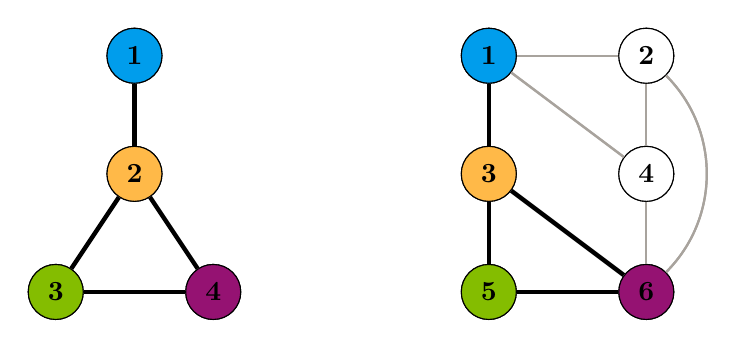
\begin{tikzpicture}
            \node <1> [draw, circle, fill=white, inner sep=4pt, font=\bfseries] (Na) at (1,  0) {1};
            \node <1> [draw, circle, fill=white, inner sep=4pt, font=\bfseries] (Nb) at (1, -1.5) {2};
            \node <1> [draw, circle, fill=white, inner sep=4pt, font=\bfseries] (Nc) at (0, -3) {3};
            \node <1> [draw, circle, fill=white, inner sep=4pt, font=\bfseries] (Nd) at (2, -3) {4};
            \node <2> [draw, circle, fill=uofgcobalt, inner sep=4pt, font=\bfseries] (Na) at (1,  0) {1};
            \node <2> [draw, circle, fill=uofgpumpkin, inner sep=4pt, font=\bfseries] (Nb) at (1, -1.5) {2};
            \node <2> [draw, circle, fill=uofglawn, inner sep=4pt, font=\bfseries] (Nc) at (0, -3) {3};
            \node <2> [draw, circle, fill=uofgthistle, inner sep=4pt, font=\bfseries] (Nd) at (2, -3) {4};

            \draw <1> [thick, color=uofgsandstone!50] (Na) -- (Nb);
            \draw <1> [thick, color=uofgsandstone!50] (Nb) -- (Nc);
            \draw <1> [thick, color=uofgsandstone!50] (Nc) -- (Nd);
            \draw <1> [thick, color=uofgsandstone!50] (Nb) -- (Nd);
            \draw <2> [ultra thick] (Na) -- (Nb);
            \draw <2> [ultra thick] (Nb) -- (Nc);
            \draw <2> [ultra thick] (Nc) -- (Nd);
            \draw <2> [ultra thick] (Nb) -- (Nd);

            \node <1> [draw, circle, fill=white, inner sep=4pt, font=\bfseries] (N1) at (5.5,  0) {1};
            \node <1> [draw, circle, fill=white, inner sep=4pt, font=\bfseries] (N2) at (7.5,  0) {2};
            \node <1> [draw, circle, fill=white, inner sep=4pt, font=\bfseries] (N3) at (5.5, -1.5) {3};
            \node <1> [draw, circle, fill=white, inner sep=4pt, font=\bfseries] (N4) at (7.5, -1.5) {4};
            \node <1> [draw, circle, fill=white, inner sep=4pt, font=\bfseries] (N5) at (5.5, -3) {5};
            \node <1> [draw, circle, fill=white, inner sep=4pt, font=\bfseries] (N6) at (7.5, -3) {6};
            \node <2> [draw, circle, fill=uofgcobalt, inner sep=4pt, font=\bfseries] (N1) at (5.5,  0) {1};
            \node <2> [draw, circle, fill=white, inner sep=4pt, font=\bfseries] (N2) at (7.5,  0) {2};
            \node <2> [draw, circle, fill=uofgpumpkin, inner sep=4pt, font=\bfseries] (N3) at (5.5, -1.5) {3};
            \node <2> [draw, circle, fill=white, inner sep=4pt, font=\bfseries] (N4) at (7.5, -1.5) {4};
            \node <2> [draw, circle, fill=uofglawn, inner sep=4pt, font=\bfseries] (N5) at (5.5, -3) {5};
            \node <2> [draw, circle, fill=uofgthistle, inner sep=4pt, font=\bfseries] (N6) at (7.5, -3) {6};

            \draw <1> [thick, color=uofgsandstone!50] (N1) -- (N2);
            \draw <1> [thick, color=uofgsandstone!50] (N1) -- (N3);
            \draw <1> [thick, color=uofgsandstone!50] (N1) -- (N4);
            \draw <1> [thick, color=uofgsandstone!50] (N2) -- (N4);
            \draw <1> [thick, color=uofgsandstone!50] (N3) -- (N5);
            \draw <1> [thick, color=uofgsandstone!50] (N3) -- (N6);
            \draw <1> [thick, color=uofgsandstone!50] (N4) -- (N6);
            \draw <1> [thick, color=uofgsandstone!50] (N5) -- (N6);
            \draw <1> [thick, color=uofgsandstone!50] (N2) to [in=45, out=315] (N6);
            \draw <2> [thick, color=uofgsandstone!50] (N1) -- (N2);
            \draw <2> [ultra thick] (N1) -- (N3);
            \draw <2> [thick, color=uofgsandstone!50] (N1) -- (N4);
            \draw <2> [thick, color=uofgsandstone!50] (N2) -- (N4);
            \draw <2> [ultra thick] (N3) -- (N5);
            \draw <2> [ultra thick] (N3) -- (N6);
            \draw <2> [thick, color=uofgsandstone!50] (N4) -- (N6);
            \draw <2> [ultra thick] (N5) -- (N6);
            \draw <2> [thick, color=uofgsandstone!50] (N2) to [in=45, out=315] (N6);
        \end{tikzpicture}\end{center}
    }

    \only<3>{
        \begin{itemize}
            \item Find an \emph{injective} mapping from a \emph{pattern} graph to a \emph{target} graph.
            \item \textbf{Adjacent} vertices must be \textbf{mapped to adjacent} vertices.
            \item For the \emph{induced} problem variant, non-adjacent vertices
                must be mapped to non-adjacent vertices.
        \end{itemize}
    }

\end{frame}

\begin{frame}{The Maximum Clique Problem}
    \begin{center}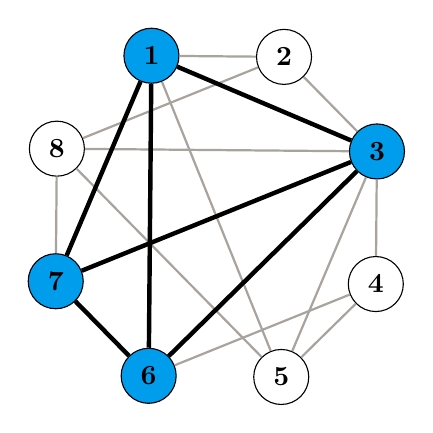
\begin{tikzpicture}
        \newcount \c
        \foreach \n in {1, ..., 8}{
            \c=\n \advance\c by -1 \multiply\c by -360 \divide\c by 8 \advance\c by 112.5
            \ifthenelse{\n = 1 \OR \n = 3 \OR \n = 6 \OR \n = 7}{
                \node[draw, circle, fill=uofgcobalt, inner sep=4pt, font=\bfseries] (N\n) at (\the\c:2.2) {\n};
            }{
                \node[draw, circle, fill=white, inner sep=4pt, font=\bfseries] (N\n) at (\the\c:2.2) {\n};
            }
        }

        \draw [thick, color=uofgsandstone!50] (N1) -- (N2);
        \draw [thick, color=uofgsandstone!50] (N1) -- (N5);
        \draw [thick, color=uofgsandstone!50] (N2) -- (N3);
        \draw [thick, color=uofgsandstone!50] (N2) -- (N8);
        \draw [thick, color=uofgsandstone!50] (N3) -- (N4);
        \draw [thick, color=uofgsandstone!50] (N3) -- (N5);
        \draw [thick, color=uofgsandstone!50] (N3) -- (N8);
        \draw [thick, color=uofgsandstone!50] (N4) -- (N5);
        \draw [thick, color=uofgsandstone!50] (N4) -- (N6);
        \draw [thick, color=uofgsandstone!50] (N5) -- (N8);
        \draw [thick, color=uofgsandstone!50] (N7) -- (N8);

        \draw [ultra thick] (N1) -- (N3);
        \draw [ultra thick] (N1) -- (N6);
        \draw [ultra thick] (N1) -- (N7);
        \draw [ultra thick] (N3) -- (N6);
        \draw [ultra thick] (N3) -- (N7);
        \draw [ultra thick] (N6) -- (N7);
    \end{tikzpicture}\end{center}

\end{frame}

\begin{frame}{Maximum Common Subgraph}
    \begin{center}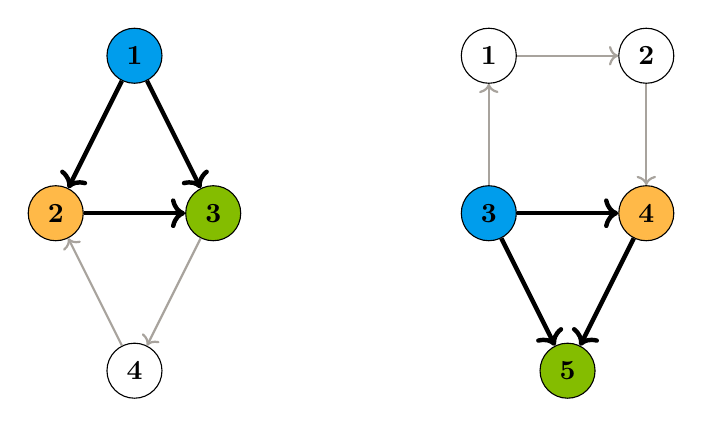
\begin{tikzpicture}%{{{
        \node[draw, circle, fill=uofgcobalt, inner sep=4pt, font=\bfseries] (Ma) at (1, -7.5) {1};
        \node[draw, circle, fill=uofgpumpkin, inner sep=4pt, font=\bfseries] (Mb) at (0, -9.5) {2};
        \node[draw, circle, fill=uofglawn, inner sep=4pt, font=\bfseries] (Mc) at (2, -9.5) {3};
        \node[draw, circle, fill=white, inner sep=4pt, font=\bfseries] (Md) at (1, -11.5) {4};

        \node[draw, circle, fill=white, inner sep=4pt, font=\bfseries] (M1) at (5.5, -7.5) {1};
        \node[draw, circle, fill=white, inner sep=4pt, font=\bfseries] (M2) at (7.5, -7.5) {2};
        \node[draw, circle, fill=uofgcobalt, inner sep=4pt, font=\bfseries] (M3) at (5.5, -9.5) {3};
        \node[draw, circle, fill=uofgpumpkin, inner sep=4pt, font=\bfseries] (M4) at (7.5, -9.5) {4};
        \node[draw, circle, fill=uofglawn, inner sep=4pt, font=\bfseries] (M5) at (6.5, -11.5) {5};

        \draw [->, thick, color=uofgsandstone!50] (Mc) -> (Md);
        \draw [->, thick, color=uofgsandstone!50] (Md) -- (Mb);
        \draw [->, ultra thick] (Ma) -> (Mb);
        \draw [->, ultra thick] (Mb) -> (Mc);
        \draw [->, ultra thick] (Ma) -> (Mc);

        \draw [->, thick, color=uofgsandstone!50] (M1) -> (M2);
        \draw [->, thick, color=uofgsandstone!50] (M2) -> (M4);
        \draw [->, thick, color=uofgsandstone!50] (M3) -> (M1);
        \draw [->, ultra thick] (M3) -> (M4);
        \draw [->, ultra thick] (M3) -> (M5);
        \draw [->, ultra thick] (M4) -> (M5);
    \end{tikzpicture}\end{center}
\end{frame}

\begin{frame}{Maximum Common Connected Subgraph?}

    \begin{columns}
        \begin{column}{0.45\textwidth}
            \centering
            \chemfig{*6(-=(-[7]N(-[5]H)(-[7]H))-=-=)}
        \end{column}
        \begin{column}{0.45\textwidth}
            \centering
            \chemfig{*6(-=(-[7]O-[7]N(-[5]H)(-[7]H))-=-=)}
        \end{column}
    \end{columns}

\end{frame}

\section{Practical Algorithms}

\begin{frame}{Who Cares?}
    \begin{columns}
        \begin{column}{0.45\textwidth}
            \begin{itemize}
                \item Bioinformatics
                \item Chemistry
                \item Drug design
                \item Computer vision
                \item Pattern recognition
                \item Financial fraud detection
                \item Model checking
                \item Fault detection
            \end{itemize}
        \end{column}
        \begin{column}{0.45\textwidth}
            \begin{itemize}
                \item Law enforcement
                \item Kidney exchange
                \item Social network analysis
                \item Compilers
                \item Diseased cows
                \item Computer algebra
                \item Circuit design
                \item Network design
            \end{itemize}
        \end{column}
    \end{columns}
\end{frame}

\begin{frame}{Practical Algorithms}
    \begin{itemize}
        \item Real-world inputs rarely have nice properties (low treewidth, particular degree
            spreads that are polynomial, etc).

        \item We can still solve some subgraph isomorphism problems with \textbf{thousand vertex
            patterns} and \textbf{ten thousand vertex targets} in a few seconds.

        \item Worst-case analysis is useless, and constant factors matter.
    \end{itemize}
\end{frame}

\begin{frame}{Constraint Models}
    \begin{itemize}
        \item We have some \textbf{variables}, each with a \textbf{domain}, and we want to give each
            variable a value from its domain.
            \begin{itemize}
                \item Subgraph isomorphism: a variable for each pattern vertex, with domains being
                    target vertices.
                \item Clique: a boolean variable for each vertex.
            \end{itemize}
        \item There are \textbf{constraints} between variables.
            \begin{itemize}
                \item Subgraph isomorphism: all-different (injectivity), and adjacent pairs of
                    vertices must be mapped to adjacent pairs of vertices.
                \item Clique: for each pair of non-adjacent vertices, at least one of the two
                    variables must be false.
            \end{itemize}
        \item There is an \textbf{objective}.
            \begin{itemize}
                \item Subgraph isomorphism: give each variable a value.
                \item Maximum clique: set as many variables to true as possible.
            \end{itemize}
    \end{itemize}
\end{frame}

\begin{frame}{Inference}
    \begin{itemize}
        \item We want to \textbf{cross out values} from domains, until only one value is left in
            each.
        \item Subgraph isomorphism: high degree vertices cannot be mapped to low degree vertices.
        \item If an assignment becomes forced, we can \textbf{infer additional deletions}. This can
            have a cascade effect.
    \end{itemize}
\end{frame}

\begin{frame}{Implied Constraints for Subgraph Isomorphism}
    \only<1> {
        \begin{itemize}
            \item Adjacent vertices must be mapped to adjacent vertices.
            \item Vertices that are distance 2 apart must be mapped to vertices that are within
                distance 2.
            \item Vertices that are distance $k$ apart must be mapped to vertices that are within
                distance $k$.
        \end{itemize}

        \vspace{1em}

        \centering
        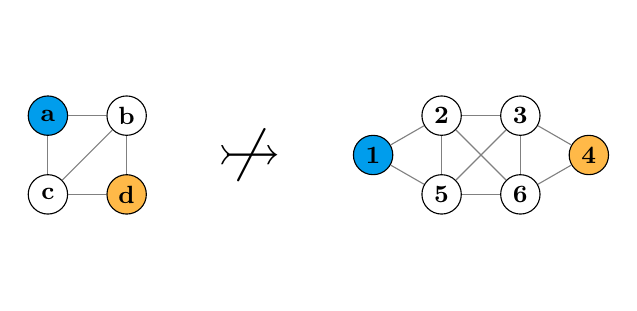
\begin{tikzpicture}
            \node [vertex] (Pc) at (0, 0) { c };
            \node [vertexc3] (Pd) at (1, 0) { d };
            \node [vertex] (Pb) at (1, 1) { b };
            \node [vertexc1] (Pa) at (0, 1) { a };

            \draw [edge] (Pa) -- (Pb);
            \draw [edge] (Pb) -- (Pc);
            \draw [edge] (Pc) -- (Pd);
            \draw [edge] (Pd) -- (Pb);
            \draw [edge] (Pa) -- (Pc);

            \node [anchor=center, font=\huge] at (2.565, 0.5) { $\centernot\rightarrowtail$ };

            \node [vertexc1] (T1) at (4.13, 0.5) { 1 };
            \node [vertex] (T5) at (5, 0) { 5 };
            \node [vertex] (T6) at (6, 0) { 6 };
            \node [vertex] (T3) at (6, 1) { 3 };
            \node [vertex] (T2) at (5, 1) { 2 };
            \node [vertexc3] (T4) at (6.87, 0.5) { 4 };

            \draw [edge] (T1) -- (T2);
            \draw [edge] (T1) -- (T5);
            \draw [edge] (T4) -- (T3);
            \draw [edge] (T4) -- (T6);
            \draw [edge] (T2) -- (T6);
            \draw [edge] (T2) -- (T3);
            \draw [edge] (T3) -- (T5);
            \draw [edge] (T5) -- (T6);
            \draw [edge] (T3) -- (T6);
            \draw [edge] (T2) -- (T5);

            \node at (5, 2) { ~ };
            \node at (5, -1) { ~ };
        \end{tikzpicture}
        \vspace{1em}
    }

    \only<2> {
        \begin{itemize}
            \item $G^d$ is the graph with the same vertex set as $G$, and an edge between $v$ and
                $w$ if the distance between $v$ and $w$ in $G$ is at most $d$.

            \item For any $d$, a subgraph isomorphism $i : P \rightarrowtail T$ is also a
                subgraph isomorphism $i^d : P^d \rightarrowtail T^d$.
        \end{itemize}

        \vspace{1em}

        \centering
        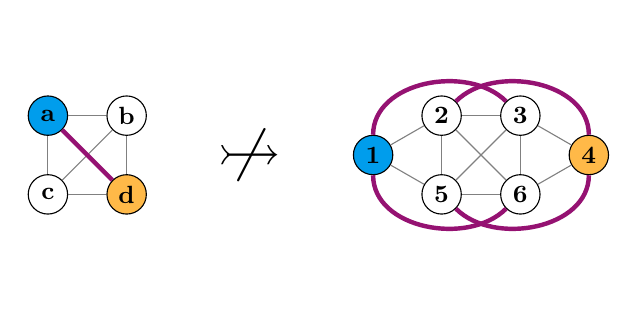
\begin{tikzpicture}
            \node [vertex] (Pc) at (0, 0) { c };
            \node [vertexc3] (Pd) at (1, 0) { d };
            \node [vertex] (Pb) at (1, 1) { b };
            \node [vertexc1] (Pa) at (0, 1) { a };

            \draw [edge] (Pa) -- (Pb);
            \draw [edge] (Pb) -- (Pc);
            \draw [edge] (Pc) -- (Pd);
            \draw [edge] (Pd) -- (Pb);
            \draw [edge] (Pa) -- (Pc);

            \draw [edgel3] (Pa) -- (Pd);

            \node [anchor=center, font=\huge] at (2.565, 0.5) { $\centernot\rightarrowtail$ };

            \node [vertexc1] (T1) at (4.13, 0.5) { 1 };
            \node [vertex] (T5) at (5, 0) { 5 };
            \node [vertex] (T6) at (6, 0) { 6 };
            \node [vertex] (T3) at (6, 1) { 3 };
            \node [vertex] (T2) at (5, 1) { 2 };
            \node [vertexc3] (T4) at (6.87, 0.5) { 4 };

            \draw [edge] (T1) -- (T2);
            \draw [edge] (T1) -- (T5);
            \draw [edge] (T4) -- (T3);
            \draw [edge] (T4) -- (T6);
            \draw [edge] (T2) -- (T6);
            \draw [edge] (T2) -- (T3);
            \draw [edge] (T3) -- (T5);
            \draw [edge] (T5) -- (T6);
            \draw [edge] (T3) -- (T6);
            \draw [edge] (T2) -- (T5);

            \draw [edgel3] (T1) to [in=135, out=90] (T3);
            \draw [edgel3] (T1) to [in=225, out=270] (T6);

            \draw [edgel3] (T4) to [in=45, out=90] (T2);
            \draw [edgel3] (T4) to [in=315, out=270] (T5);

            \node at (5, 2) { ~ };
            \node at (5, -1) { ~ };
        \end{tikzpicture}
        \vspace{1em}
    }

    \only<3> {
        \begin{itemize}
            \item We can do something stronger: rather than looking at distances, we can look at
                \textbf{(simple) paths}, and we can count how many there are.

            \item This is \NP-hard in general, but only lengths 2 and 3 and counts of 2 and 3 are
                useful in practice.

            \item We construct these graph pairs once, at the top of search.

            \item We can also use these graph pairs for degree-based filtering.
        \end{itemize}
    }

\end{frame}

\begin{frame}{Search}
    \begin{itemize}
        \item Sometimes we have to \textbf{guess}: pick a variable $x$. Then for each value $v_i$ in
            its domain in turn, see what happens if we force $x = v_i$.
        \item There are good heuristics telling us which variable to pick first.
        \item There are heuristics telling us which value to pick first, but this seems to be
            less reliable in general.
    \end{itemize}
\end{frame}

\begin{frame}{Branch and Bound}

    \begin{center}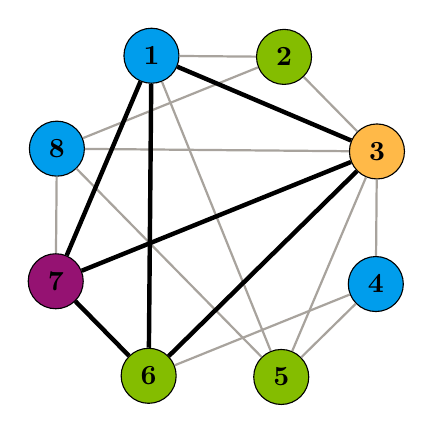
\begin{tikzpicture}
        \newcount \c
        \foreach \n in {1, ..., 8}{
            \c=\n \advance\c by -1 \multiply\c by -360 \divide\c by 8 \advance\c by 112.5
            \ifthenelse{\n = 1 \OR \n = 4 \OR \n = 8}{
                \node[draw, circle, fill=uofgcobalt, inner sep=4pt, font=\bfseries] (N\n) at (\the\c:2.2) {\n};
            }{}
            \ifthenelse{\n = 2 \OR \n = 5 \OR \n = 6}{
                \node[draw, circle, fill=uofglawn, inner sep=4pt, font=\bfseries] (N\n) at (\the\c:2.2) {\n};
            }{}
            \ifthenelse{\n = 3}{
                \node[draw, circle, fill=uofgpumpkin, inner sep=4pt, font=\bfseries] (N\n) at (\the\c:2.2) {\n};
            }{}
            \ifthenelse{\n = 7}{
                \node[draw, circle, fill=uofgthistle, inner sep=4pt, font=\bfseries] (N\n) at (\the\c:2.2) {\n};
            }{}
        }

        \draw [thick, color=uofgsandstone!50] (N1) -- (N2);
        \draw [thick, color=uofgsandstone!50] (N1) -- (N5);
        \draw [thick, color=uofgsandstone!50] (N2) -- (N3);
        \draw [thick, color=uofgsandstone!50] (N2) -- (N8);
        \draw [thick, color=uofgsandstone!50] (N3) -- (N4);
        \draw [thick, color=uofgsandstone!50] (N3) -- (N5);
        \draw [thick, color=uofgsandstone!50] (N3) -- (N8);
        \draw [thick, color=uofgsandstone!50] (N4) -- (N5);
        \draw [thick, color=uofgsandstone!50] (N4) -- (N6);
        \draw [thick, color=uofgsandstone!50] (N5) -- (N8);
        \draw [thick, color=uofgsandstone!50] (N7) -- (N8);

        \draw [ultra thick] (N1) -- (N3);
        \draw [ultra thick] (N1) -- (N6);
        \draw [ultra thick] (N1) -- (N7);
        \draw [ultra thick] (N3) -- (N6);
        \draw [ultra thick] (N3) -- (N7);
        \draw [ultra thick] (N6) -- (N7);
    \end{tikzpicture}\end{center}

    \begin{itemize}
        \item For optimisation: keep track of the \textbf{best solution} we've found so far. If we can show
            we can't beat it, backtrack immediately.
    \end{itemize}

\end{frame}

\begin{frame}{Backjumping}

    \begin{itemize}
        \item When backtracking, see if the current assignment actually removed any values which
            could have helped prevent the failure. If not, \textbf{jump back} another step.
    \end{itemize}

\end{frame}

\begin{frame}{Is This Any Good?}

    \input{gen-graph-ecdf}

\end{frame}

\section{Phase Transitions}

\begin{frame}{Generating Hard Subgraph Isomorphism Instances}

    \begin{itemize}
        \item We can solve some problem instances with a thousand pattern vertices, and ten thousand
            target vertices. Can we solve \emph{any} instance with these sizes?

        \item We like having \textbf{lots of instances}, to make sure we don't overfit algorithm
            parameters.

        \item How do we create random subgraph isomorphism instances?
    \end{itemize}

\end{frame}

\begin{frame}{Phase Transitions in Non-Induced Subgraph Isomorphism}

    \input{gen-graph-phase-transition}

\end{frame}

\begin{frame}{This Looks Familiar\ldots}
    \centering
    \includegraphics*[keepaspectratio=true,scale=0.25]{sat.jpg}

    \par\flushleft
    Understanding the Empirical Hardness of NP-Complete Problems. Kevin Leyton-Brown, Holger H.
    Hoos, Frank Hutter, Lin Xu.  Communications of the ACM, Vol. 57 No. 5, Pages 98-107
\end{frame}

\begin{frame}{Varying Both Densities?}
    \only<1> {
        \input{gen-graph-non-induced-1}
    }

    \only<2> {
        \input{gen-graph-non-induced-2}
    }

    \only<3> {
        \input{gen-graph-non-induced-3}
    }
\end{frame}

\begin{frame}{Heuristics from Maximising Expectations}

    \only<1> {
        \begin{itemize}
            \item With a few dubious assumptions regarding independence and integers, the expected
                number of solutions is \[ \langle Sol \rangle = t \cdot (t - 1) \cdot \ldots
                        \cdot (t - p + 1) \cdot {d_t}^{d_p \cdot \binom{p}{2}} \textnormal{.} \]
            \item If $\langle Sol \rangle \ll 1$, the instance is likely to be unsatisfiable.
            \item Unfortunately, if $\langle Sol \rangle \gg 1$, things are a bit trickier\ldots
        \end{itemize}
    }

    \only<2> {
        \input{gen-graph-non-induced-prediction}
    }

    \only<3> {
        \begin{itemize}
            \item Suppose we wanted to maximise the expected number of solutions in a subproblem during
                search. \\[0.3cm]

        \end{itemize}
        {\Large \[ \langle Sol \rangle = \tikzmark{sdfstart}t \cdot (t - 1) \cdot \ldots \cdot (t -
                p + 1)\tikzmark{sdfend} \, \cdot \,
                {\tikzmark{targetstart}d_t\tikzmark{targetend}
                ~}^{\, d_p ~ \cdot ~ \binom{p}{2}}\tikzmark{patternend}
        \] \\[0.5cm]}

        
\begin{tikzpicture}[remember picture, overlay]
            \draw [decorate, decoration={brace, mirror, raise=0.2cm}, thick] (pic cs:sdfstart) --
            (pic cs:sdfend) node [midway, below=0.3cm] { smallest domain };

            \draw [decorate, decoration={brace, mirror, raise=0.2cm}, thick] (pic cs:targetstart) --
            (pic cs:targetend) node [midway, below=0.3cm, text width=3em, align=center] { low degree };

            \draw [decorate, decoration={brace, mirror, raise=0.2cm}, thick] ($(pic
            cs:targetend)+(0.3,0)$) -- (pic cs:patternend) node [midway, below=0.3cm, text width=4em, align=center] { high degree };
        \end{tikzpicture}

        \begin{itemize}
            \item These heuristics are used in practice (sort of), but were discovered through
                guessing and experiments!
        \end{itemize}
    }

\end{frame}

\begin{frame}{Phase Transitions in Induced Subgraph Isomorphism}

    \only<1> {
        \input{gen-graph-induced-1}
    }

    \only<2> {
        \input{gen-graph-induced-2}
    }

    \only<3> {
        \input{gen-graph-induced-3}
    }

\end{frame}

\begin{frame}{Can We Predict This?}

    \only<1> {
        \begin{itemize}
            \item With a few more dubious assumptions, the expected
                number of solutions is now \[ \langle Sol \rangle = t \cdot (t - 1) \cdot \ldots
                    \cdot (t - p + 1) \cdot {d_t}^{d_p \cdot \binom{p}{2}} \cdot {(1 - d_t)}^{(1 -
                        d_p) \cdot \binom{p}{2}} \textnormal{.} \]
        \end{itemize}
    }

    \only<2> {
        \input{gen-graph-induced-prediction}
    }
\end{frame}

\begin{frame}{Why is the Middle Region Hard?}

    \only<1> {
        \centering
        \input{gen-graph-induced-reduction}
    }

    \only<2> {
        \input{gen-graph-induced-kappa}
    }

\end{frame}

\begin{frame}{Induced Heuristics?}

    \only<1> {
        \begin{itemize}
            \item For anything we say about degree, the opposite holds for the complement constraints.

            \item Degree-based value ordering heuristics don't seem to help. This is intuitive, but
                does this formula give us a heuristic after all?
        \end{itemize}
    }

    \only<2> {
        \input{gen-graph-induced-heuristic}
    }
\end{frame}

\section{Parallelism}

\begin{frame}{Thread-Parallel Tree Search}

    \only<1-3> {
        \centering
        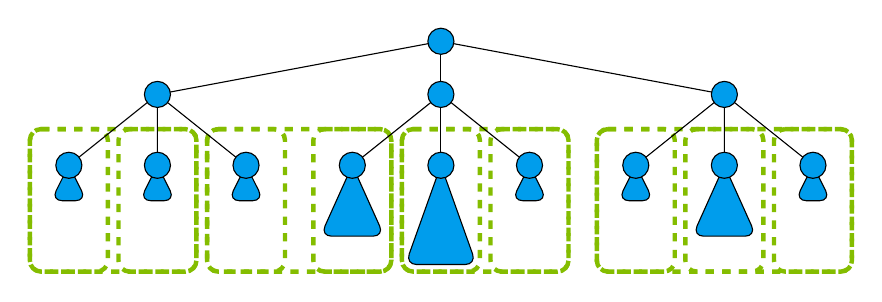
\begin{tikzpicture}[scale=0.9]%{{{
            \coordinate (R);

            \coordinate (N) at (R);

            \coordinate (N1) at ($(N) + (-4, -0.75)$);
            \coordinate (N2) at ($(N) + ( 0, -0.75)$);
            \coordinate (N3) at ($(N) + ( 4, -0.75)$);

            \foreach \na in {1, ..., 3}{
                \coordinate (N\na 1) at ($(N\na) + (-1.25, -1)$);
                \coordinate (N\na 2) at ($(N\na) + ( 0,    -1)$);
                \coordinate (N\na 3) at ($(N\na) + ( 1.25, -1)$);

                \foreach \nb in {1, ..., 3}{
                    \coordinate (N\na\nb t1) at ($(N\na\nb) + (-0.45, -1)$);
                    \coordinate (N\na\nb t2) at ($(N\na\nb) + ( 0.45, -1)$);

                    \coordinate (N\na\nb s1) at ($(N\na\nb) + (-0.25, -0.5)$);
                    \coordinate (N\na\nb s2) at ($(N\na\nb) + ( 0.25, -0.5)$);

                    \coordinate (N\na\nb h1) at ($(N\na\nb) + (-0.5, -1.4)$);
                    \coordinate (N\na\nb h2) at ($(N\na\nb) + ( 0.5, -1.4)$);
                }
            }

            \tikzstyle{i} = [draw, rounded corners, dashed, color=white, ultra thick];
            \draw <1> [i] ($(N11) + (-0.55, 0.51)$) -- ($(N12) + (0.55, 0.51)$) -- ($(N12) + (0.55, -1.5)$) -- ($(N11) + (-0.55, -1.5)$) -- cycle;
            \draw <1> [i] ($(N13) + (-0.55, 0.51)$) -- ($(N21) + (0.55, 0.51)$) -- ($(N21) + (0.55, -1.5)$) -- ($(N13) + (-0.55, -1.5)$) -- cycle;
            \draw <1> [i] ($(N22) + (-0.55, 0.51)$) -- ($(N23) + (0.55, 0.51)$) -- ($(N23) + (0.55, -1.5)$) -- ($(N22) + (-0.55, -1.5)$) -- cycle;
            \draw <1> [i] ($(N31) + (-0.55, 0.51)$) -- ($(N33) + (0.55, 0.51)$) -- ($(N33) + (0.55, -1.5)$) -- ($(N31) + (-0.55, -1.5)$) -- cycle;

            \tikzstyle{p} = [draw, rounded corners, dashed, color=uofglawn, ultra thick];
            \draw <2> [p] ($(N11) + (-0.55, 0.51)$) -- ($(N12) + (0.55, 0.51)$) -- ($(N12) + (0.55, -1.5)$) -- ($(N11) + (-0.55, -1.5)$) -- cycle;
            \draw <2> [p] ($(N13) + (-0.55, 0.51)$) -- ($(N21) + (0.55, 0.51)$) -- ($(N21) + (0.55, -1.5)$) -- ($(N13) + (-0.55, -1.5)$) -- cycle;
            \draw <2> [p] ($(N22) + (-0.55, 0.51)$) -- ($(N23) + (0.55, 0.51)$) -- ($(N23) + (0.55, -1.5)$) -- ($(N22) + (-0.55, -1.5)$) -- cycle;
            \draw <2> [p] ($(N31) + (-0.55, 0.51)$) -- ($(N33) + (0.55, 0.51)$) -- ($(N33) + (0.55, -1.5)$) -- ($(N31) + (-0.55, -1.5)$) -- cycle;

            \foreach \na in {1, ..., 3}{
                \foreach \nb in {1, ..., 3}{
                    \draw <3> [p] ($(N\na\nb) + (-0.55, 0.51)$) -- ($(N\na\nb) + (0.55, 0.51)$) --
                    ($(N\na\nb) + (0.55, -1.5)$) -- ($(N\na\nb) + (-0.55, -1.5)$) -- cycle;
                }
            }

            \foreach \na in {1, ..., 3}{
                \draw (N) -- (N\na);
                \foreach \nb in {1, ..., 3}{
                    \draw (N\na) -- (N\na\nb);
                }
            }

            \tikzstyle{t} = [draw, fill, fill=uofgcobalt, rounded corners];

            \draw [t] (N11) -- (N11s1) -- (N11s2) -- cycle;
            \draw [t] (N12) -- (N12s1) -- (N12s2) -- cycle;
            \draw [t] (N13) -- (N13s1) -- (N13s2) -- cycle;

            \draw [t] (N21) -- (N21t1) -- (N21t2) -- cycle;
            \draw [t] (N22) -- (N22h1) -- (N22h2) -- cycle;
            \draw [t] (N23) -- (N23s1) -- (N23s2) -- cycle;

            \draw [t] (N31) -- (N31s1) -- (N31s2) -- cycle;
            \draw [t] (N32) -- (N32t1) -- (N32t2) -- cycle;
            \draw [t] (N33) -- (N33s1) -- (N33s2) -- cycle;

            \tikzstyle{c} = [draw, circle, fill, fill=uofgcobalt];
            \node [c] at (N) { };

            \foreach \na in {1, ..., 3}{
                \node [c] at (N\na) { };

                \foreach \nb in {1, ..., 3}{
                    \node [c] at (N\na\nb) { };
                }
            }
        \end{tikzpicture}%}}}
    }

\end{frame}

\begin{frame}{Parallel Search Order Matters}

    \only<1-2> {
        \centering
        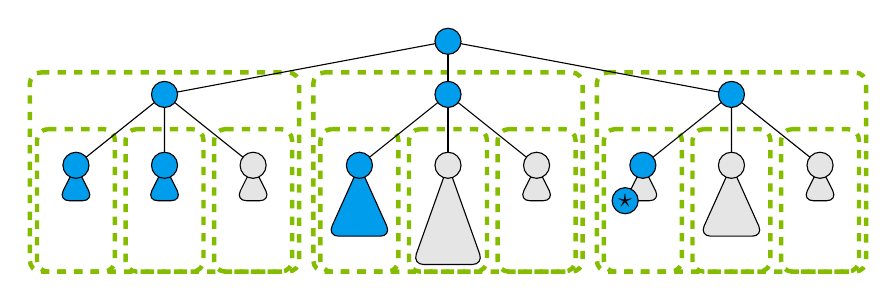
\begin{tikzpicture}[scale=0.9]%{{{
            \coordinate (R);

            \coordinate (N) at (R);

            \coordinate (N1) at ($(N) + (-4, -0.75)$);
            \coordinate (N2) at ($(N) + ( 0, -0.75)$);
            \coordinate (N3) at ($(N) + ( 4, -0.75)$);


            \foreach \na in {1, ..., 3}{
                \coordinate (N\na 1) at ($(N\na) + (-1.25, -1)$);
                \coordinate (N\na 2) at ($(N\na) + ( 0,    -1)$);
                \coordinate (N\na 3) at ($(N\na) + ( 1.25, -1)$);

                \foreach \nb in {1, ..., 3}{
                    \coordinate (N\na\nb t1) at ($(N\na\nb) + (-0.45, -1)$);
                    \coordinate (N\na\nb t2) at ($(N\na\nb) + ( 0.45, -1)$);

                    \coordinate (N\na\nb s1) at ($(N\na\nb) + (-0.25, -0.5)$);
                    \coordinate (N\na\nb s2) at ($(N\na\nb) + ( 0.25, -0.5)$);

                    \coordinate (N\na\nb h1) at ($(N\na\nb) + (-0.5, -1.4)$);
                    \coordinate (N\na\nb h2) at ($(N\na\nb) + ( 0.5, -1.4)$);
                }
            }

            \tikzstyle{p} = [draw, rounded corners, dashed, color=uofglawn, ultra thick];
            \tikzstyle{q} = [draw, rounded corners, dashed, color=uofglawn, ultra thick];

            \foreach \na in {1, ..., 3}{
                \foreach \nb in {1, ..., 3}{
                    \draw <1> [p] ($(N\na\nb) + (-0.55, 0.51)$) -- ($(N\na\nb) + (0.55, 0.51)$) --
                    ($(N\na\nb) + (0.55, -1.5)$) -- ($(N\na\nb) + (-0.55, -1.5)$) -- cycle;
                }

                \draw <2> [q] ($(N\na 1) + (-0.65, 1.31)$) -- ($(N\na 3) + (0.65, 1.31)$) --
                ($(N\na 3) + (0.65, -1.5)$) -- ($(N\na 1) + (-0.65, -1.5)$) -- cycle;
            }

            \foreach \na in {1, ..., 3}{
                \draw (N) -- (N\na);
                \foreach \nb in {1, ..., 3}{
                    \draw (N\na) -- (N\na\nb);
                }
            }

            \tikzstyle{t} = [draw, fill, fill=uofgcobalt, rounded corners];
            \tikzstyle{u} = [draw, fill, fill=black!10!white, rounded corners];

            \draw [t] (N11) -- (N11s1) -- (N11s2) -- cycle;
            \draw [t] (N12) -- (N12s1) -- (N12s2) -- cycle;
            \draw [u] (N13) -- (N13s1) -- (N13s2) -- cycle;

            \draw [t] (N21) -- (N21t1) -- (N21t2) -- cycle;
            \draw [u] (N22) -- (N22h1) -- (N22h2) -- cycle;
            \draw [u] (N23) -- (N23s1) -- (N23s2) -- cycle;

            \draw [u] (N31) -- (N31s1) -- (N31s2) -- cycle;
            \draw [u] (N32) -- (N32t1) -- (N32t2) -- cycle;
            \draw [u] (N33) -- (N33s1) -- (N33s2) -- cycle;

            \tikzstyle{c} = [draw, circle, fill, fill=uofgcobalt];
            \tikzstyle{e} = [draw, circle, fill, fill=black!10!white];
            \node [c] at (N) { };

            \foreach \na in {1, ..., 3}{
                \node [c] at (N\na) { };

                \foreach \nb in {1, ..., 3}{
                    \ifthenelse{\na\nb = 11 \OR \na\nb = 12 \OR \na\nb = 21 \OR \na\nb = 31}{
                        \node [c] at (N\na\nb) { };
                    }{
                        \node [e] at (N\na\nb) { };
                    }
                }
            }

            \node [c] at (N31s1) { };
            \node at (N31s1) { $\star$ };
        \end{tikzpicture}%}}}
    }

    \only<3> {
        \centering
        \input{gen-graph-speedup}
    }

    \only<4> {
        \centering
        \input{gen-graph-speedup-2}
    }

    \only<5> {
        \centering
        \input{gen-graph-speedup-3}
    }

    \only<6> {
        \centering
        \input{gen-graph-speedup-4}
    }

    \only <7> {
        \begin{itemize}
            \item Value-ordering heuristics tend to be \textbf{worst high up} the search tree.
            \item But depth-first searches commit completely to the first choice made\ldots
            \item Discrepancy searches can avoid this problem by doing more work in total. Parallel
                search can give \textbf{similar benefits for free}.
        \end{itemize}
    }
\end{frame}

\begin{frame}{Safety and Reproducibility}

    \only<1>{
        \begin{itemize}
            \item My ``wish list'':
                \begin{enumerate}
                    \item Parallel search should \textbf{not be substantially
                        slower} than sequential search.
                    \item Adding more processors should \textbf{not make things
                        substantially worse}.
                    \item Running the same program twice on the same hardware
                        should give \textbf{similar runtimes}.
                \end{enumerate}
            \item This is surprisingly tricky.
            \item On top of all that, we want to \textbf{prioritise work stealing}
                from where we're most likely to be wrong, or possibly from where
                we're most likely not to eliminate a subtree.
        \end{itemize}
    }

\end{frame}

\begin{frame}{Parallel Search is Worth Doing}

    \only<1> {
        \vskip-5pt \input{gen-graph-speedups-scatter}
    }

    \only<2> {
        \vskip-5pt \input{gen-graph-speedups-ecdf}
    }

\end{frame}

\section{Works in Progress}

\begin{frame}{Describing and Implementing Parallel Search}

    \begin{itemize}
        \item Implementing safe and reproducible parallel search by hand, even just for multi-core,
            is painful.
        \item Current high level approaches don't offer the properties we need.
        \item Is there a better way?
    \end{itemize}

\end{frame}

\begin{frame}{Symmetries}

    \begin{itemize}
        \item Some graphs have known symmetries. Can we exploit this?

            \begin{itemize}
                \item In some ways, maximum clique is just a completely symmetric version of maximum
                    common subgraph.
            \end{itemize}

        \item What about if we have to detect the symmetries ourselves dynamically?
    \end{itemize}

\end{frame}

\begin{frame}{Explaining Failures}

    \begin{itemize}
        \item Backjumping works because when we fail, we \textbf{work out why},
            and use that to backtrack further.

        \item But then we throw that information away\ldots

        \item CNF encodings for graph problems tend to be annoyingly big, and lose structural
            information.
    \end{itemize}

\end{frame}

\begin{frame}{Graph Algorithms and Optimisation}

    \begin{itemize}
        \item There are a lot of real-world optimisation problems involving \textbf{a
            graph problem} (subgraph isomorphism, subgraph covering, finding
            sequences of related subgraphs, clique finding, graph colouring,
            \ldots), plus some \textbf{other constraints}.

        \item Can we make these problems easier to specify in a
            \textbf{high-level constraint modelling language} like \sout{Essence'}
            MiniZinc?

        \item There is a continuum of what we could do with these models:

            \begin{itemize}

                \item Compile to CP, MIP or SAT (but these models tend to be large, and lose
                    structural and heuristic information).
                \item A hybrid, multi-solver approach, ``graph morphisms modulo theories'' style
                    (but we need better theories).
                \item Compile to subgraph isomorphism (but even simple arithmetic constraints become
                    disgusting under reduction).

            \end{itemize}
    \end{itemize}

\end{frame}

\begin{frame}[plain,noframenumbering,b]
    \begin{tikzpicture}[remember picture, overlay]
        \node at (current page.north west) {
            \begin{tikzpicture}[remember picture, overlay]
                \fill [fill=uofguniversityblue, anchor=north west] (0, 0) rectangle (\paperwidth, -1.7cm);
            \end{tikzpicture}
        };

        \node (logo) [anchor=north east, shift={(-0.3cm,-0.2cm)}] at (current page.north east) {
            \includegraphics*[keepaspectratio=true,scale=0.55]{UoG_keyline.pdf}
        };
    \end{tikzpicture}

    \begin{center}
        \url{http://dcs.gla.ac.uk/~ciaran} \\
        \href{mailto:c.mccreesh.1@research.gla.ac.uk}{\nolinkurl{c.mccreesh.1@research.gla.ac.uk}}
        \\ [1cm]
    \end{center}
\end{frame}

\end{document}

